\documentclass[conference]{IEEEtran}
\IEEEoverridecommandlockouts
% The preceding line is only needed to identify funding in the first footnote. If that is unneeded, please comment it out.
\usepackage{cite}
\usepackage{amsmath,amssymb,amsfonts}
\usepackage{algorithmic}
\usepackage{graphicx}
\usepackage{textcomp}
\usepackage{xcolor}
\usepackage{hyperref}

\hypersetup{
    colorlinks=true,
    linkcolor=red,
    filecolor=magenta,      
    urlcolor=cyan,
}

\def\BibTeX{{\rm B\kern-.05em{\sc i\kern-.025em b}\kern-.08em
    T\kern-.1667em\lower.7ex\hbox{E}\kern-.125emX}}
\begin{document}

% \title{Image Processing for Analysis of Hand Drawn Multi-Loop Circuit Diagrams}
\title{Handy: Circuit Analysis of Multi Mesh Hand-Drawn Circuit Diagrams}

\author{\IEEEauthorblockN{Sara Jameel}
\IEEEauthorblockA{\textit{Habib University}\\
Karachi, Pakistan \\
sj03693@st.habib.edu.pk}
\and
\IEEEauthorblockN{Muhammad Shahrom Ali}
\IEEEauthorblockA{\textit{Habib University }\\
Karachi, Pakistan \\
ma03559@st.habib.edu.pk}
}

\maketitle

\begin{abstract}
Circuit diagrams are the prime tool in analysis of electric circuits however manually solving for current and voltage values becomes banal and unnecessarily time consuming. Over the years there have been a few attempts at automating this task. The task can be broken down into two: Circuit Recognition and Circuit Analysis. Circuit Recognition simply aims to for read the circuit from a physical medium like paper and extract component information. This can then be passed into circuit simulation tools for quick digitization of the circuit diagram. Circuit Analysis aims to read the circuit from a physical medium and solve for corresponding values of voltage and current for each circuit element. The latter has also been attempted but no prominent solutions exist for analysis of complex circuits with multiple meshes. 
\end{abstract}

\begin{IEEEkeywords}
Circuit Analysis, Image Processing, Hand drawn circuits, Mesh Analysis, Multi Mesh
\end{IEEEkeywords}

\section{\textbf{Introduction}}
Drawing a circuit diagram is one of the most common ways of solving a circuit and finding out Voltage \& Current values for each element. However, the process is tedious: formulating simultaneous equations and then solving them (Either by elimination or substitution) takes too long. And its even more difficult for an instructor to check the answers. A tool that can automate this process, taking an image as input and providing Voltage and Current values for each component would be very beneficial.

This project aims to get one step closer to automating electric circuit analysis. The system takes an image of the circuit diagram as input and outputs the Voltage and Current values of each passive element. Conventional current flow is assumed. The current implementation is limited to two mesh circuits, with 2 voltage sources and any number of resistors. However the system is designed with scaling in mind, the system solves the circuits by forming the matrix equation which allows for relatively easy scaling of the system to more meshes in the circuit. 
 

\section{\textbf{Literature Review}}
There are a bunch of solutions that already exist around this problem, but they all do part of the work or do less work. In the solution by Larik, Rehman, and Azeem \cite{SIFT}, the aim is to automate the circuit analysis process. It is an attempt to digitize hand drawn circuits and perform basic circuit analysis. A feature extraction-based method is utilized for recognition of circuit symbols which is then combined with a neural network for recognition of numerical values of components. This approach has been tested on a single mesh circuit.  \\
\noindent
The methodology used here is that an image is converted into a binarized version by applying Otsu thresholding, from an input RGB or greyscale image. Proceeding this, connecting lines are separated, numerical values and components are extracted from the image. Following this morphological processing is applied, closing is the first step that is performed on the binarized image to fulfil any gaps in the binarized image. Opening is performed to break the isthmus between the positive sign in the DC source with the inner boundary. Erosion is applied to smooth out the components so that they are more recognizable.  \\
\noindent
Numerical values in the circuit are recognized with the assistance of a pre trained neural network which has been trained on a data set of human hand written digits. The placement of the components is recognized and an equation is formulated to calculate the mesh current.\\

\noindent
 In the solution in \cite{ANNs}, an Artificial Neural Network (ANN) is used here to recognize and identify electrical devices. In the first step the image taken is binarized, after this normalization is implemented on it. Later on, using the image’s moments (Image moments identify the properties of a simple image including intensity, its centroid and orientation information.) other features of the image are extracted and then fed into the input layer of the ANN. The network then utilizes a back propagation algorithm to calculate the error with respect to the desired class. 

the moment’s extraction process includes the following steps: 

\begin{itemize}
    \item Loading image from the training data set. 
    \item Image binarization. 
    \item Image normalization.  
    \item Converting input image to a matrix. 
    \item Converting the matrix to vector of moments. 
    \item Concatenate all vectors of moments (1705) to make one matrix. 
\end{itemize}

Images in this particular method are resized to 200x200. So, the output of the conversion is a 1D array which contains moments with 220 values. \\ 

\noindent
The ANN used in this study is a feed-forward (acyclic) network. There were 1705 training samples in the input layers and 31 in hidden layers which resulted in 31 outputs after classification. 20 different hand drawn samples were used to test the procedure.\\

\noindent
The precision reported in this case is 0.8538, the recall is reported to be 0.8338 and the Fmeasure is reported to be equal to 0.8364 \\

\noindent

The method proposed by Vasudevan \cite{IP_techs}, solves the circuit for resistors, capacitors and inductors. This method solves the problem of hand written circuit recognition by using a netlist for the drawn circuit.  This netlist is created for the identified components which can be fed into the circuit analyzer. Firstly, the image is denoised by converting it into a gray scale image. This solution uses bounding rectangles to group components. Categorization is done through X Y coordinates of each bounding rectangle.  To recognize the handwritten digits, the MNIST (Mixed National Institute of Standards and Technology) database is used, symbols like ohms, micro etc. are also recognized using the MNIST dataset. Concerns or constraints of this recognition method are low lighting and poor camera quality.

\section{\textbf{Methodology}}
    The system consists of two phases: Image processing and Circuit Solving. 
    \begin{figure}[h!]
        \centering
        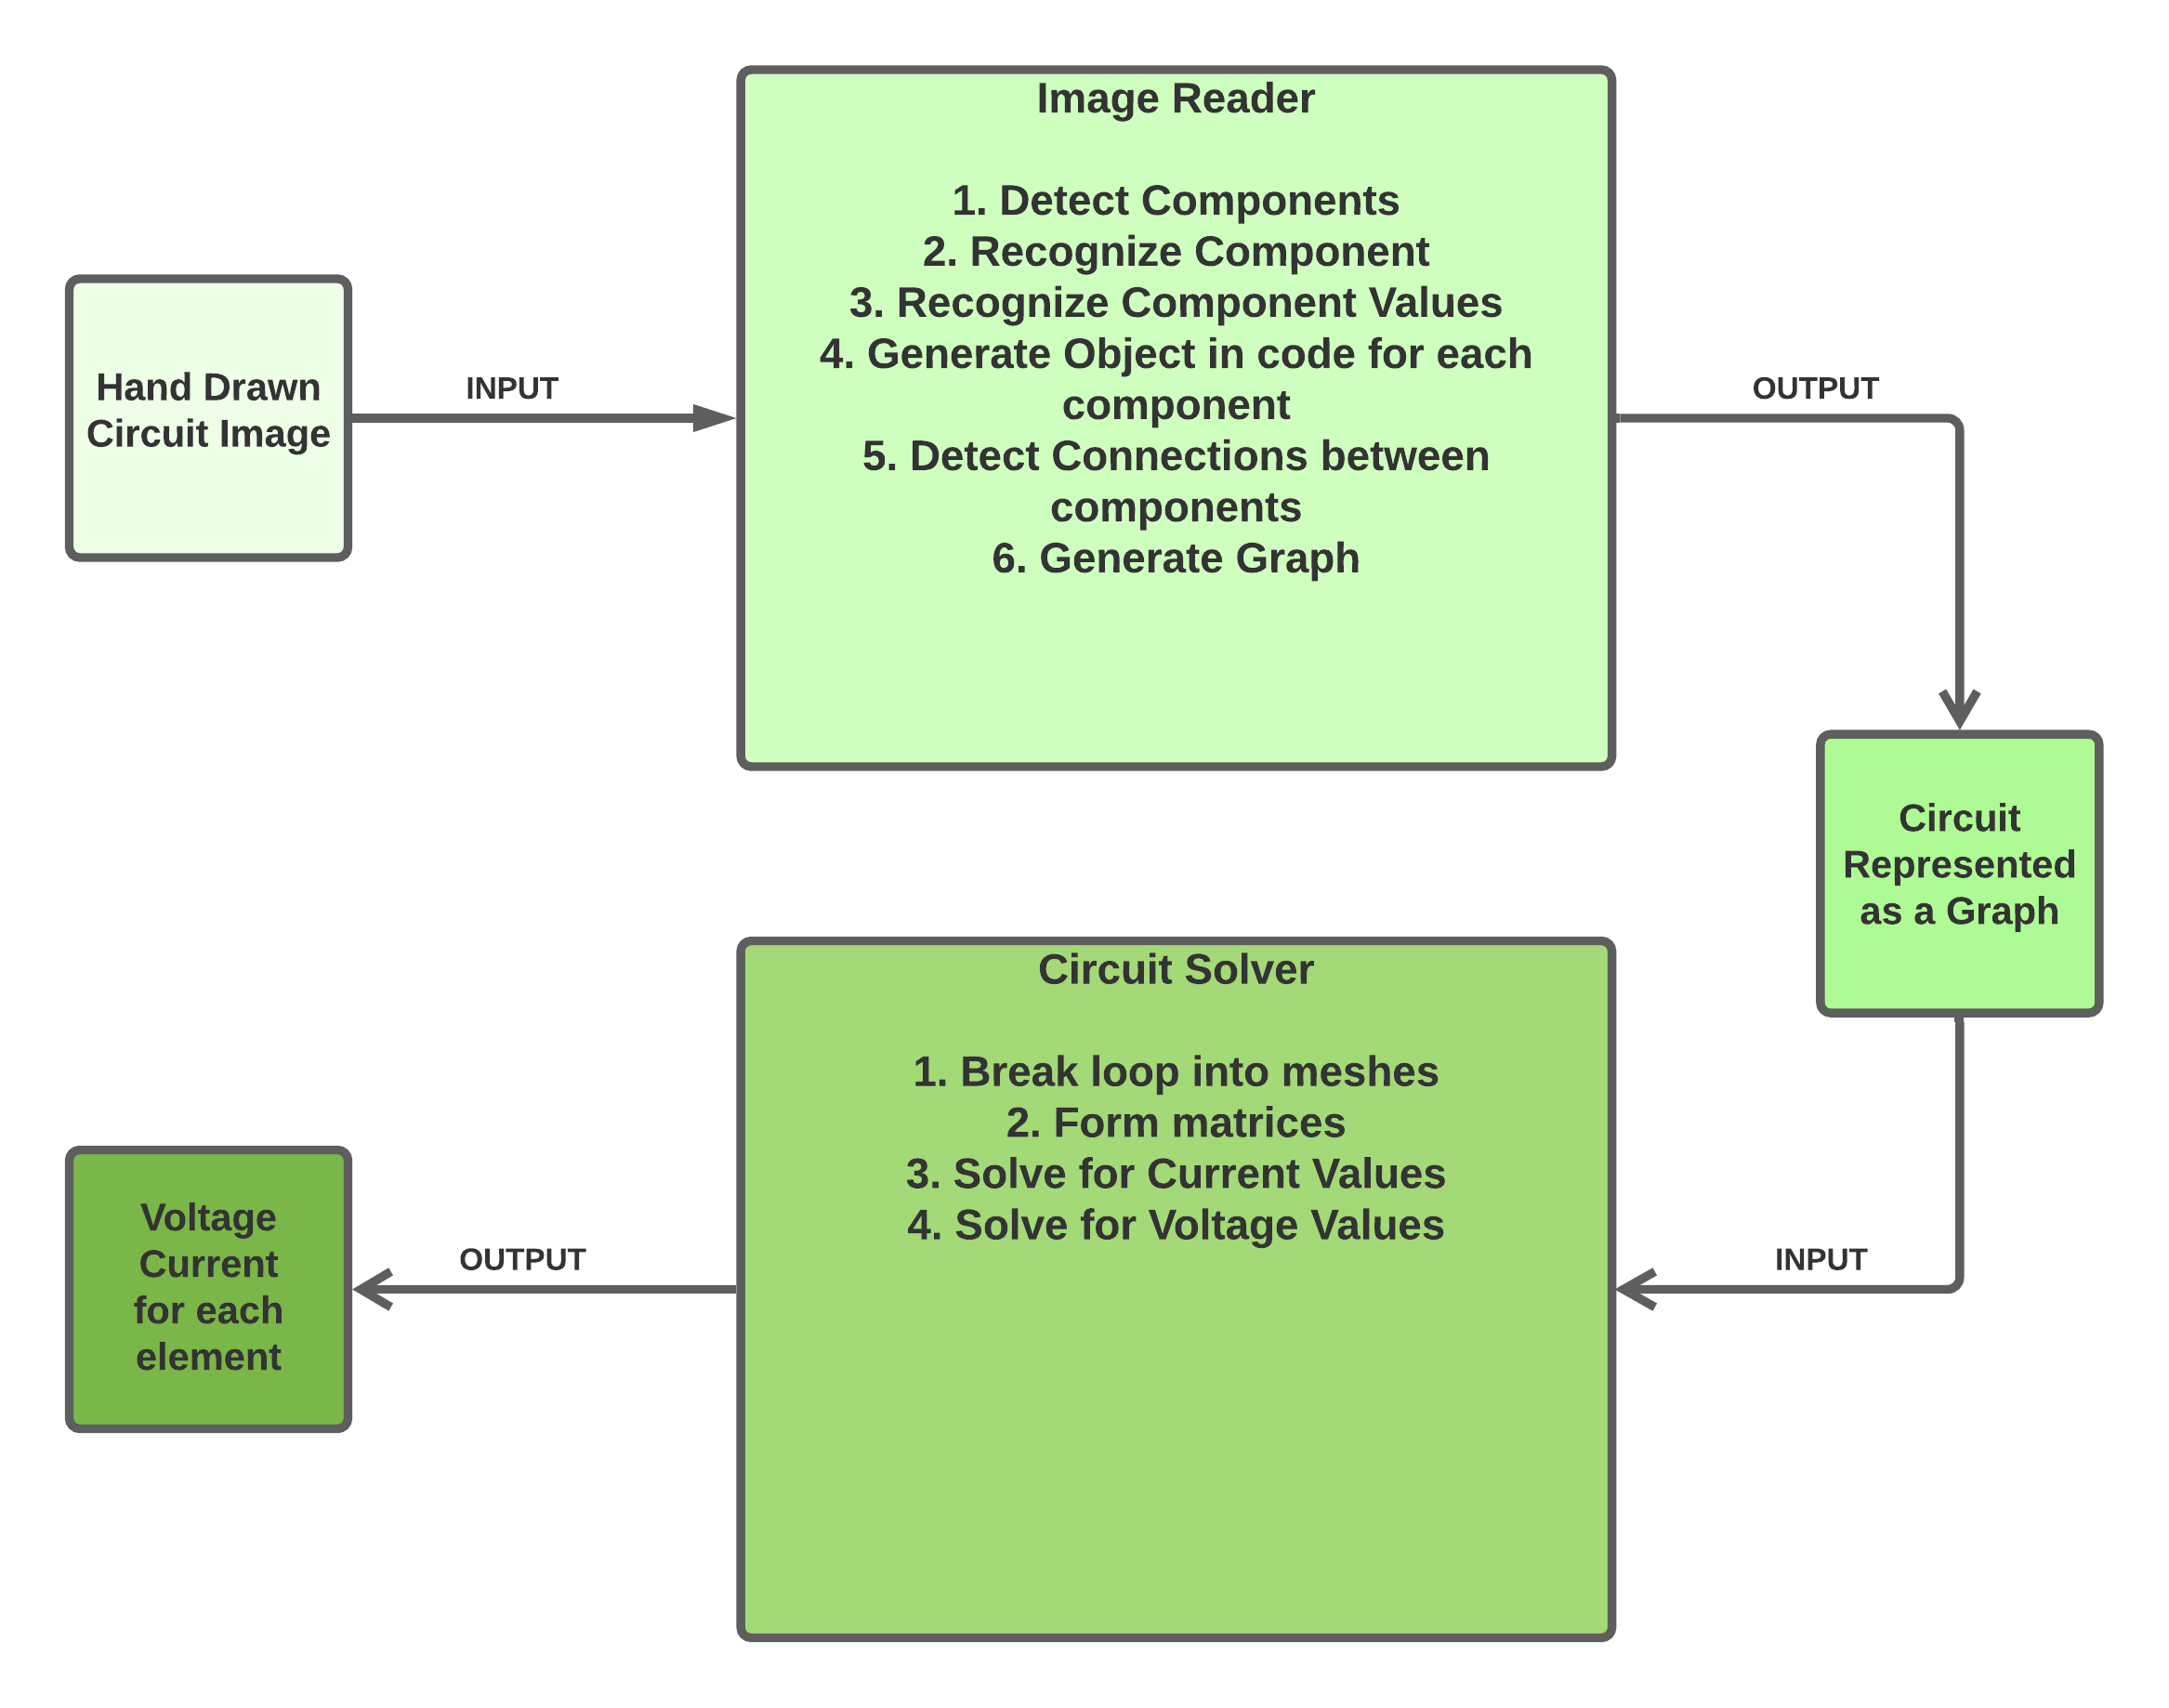
\includegraphics[scale=0.1]{images/System_Diagram.png}
        \caption{System Diagram}
        \label{fig:my_label}
    \end{figure}

    \subsection{Image Processing}
        \noindent
        \underline{Input}: Image \\
        \underline{Output}: Circuit Represented as a Graph.\\
        This step parses the image into a computer readable format. Our aim was to read circuit components and their connectivity from the image, and represent it as a directed graph (shown in figures \ref{fig:circuit_diagram} and \ref{fig:circuit_graph}). As a result, we can perform any kind of computation on all elements of the circuit, and at any meaningful point of the circuit. Moreover, this opens up the possibility of manipulating the circuit even \textit{after} reading it.    

    \begin{figure}[h!]
        \centering
        \includegraphics[scale=0.6]{images/Circuit_2.png}
        \caption{A Circuit Diagram}
        \label{fig:circuit_diagram}
    \end{figure}
    
    \begin{figure}[h!]
        \centering
        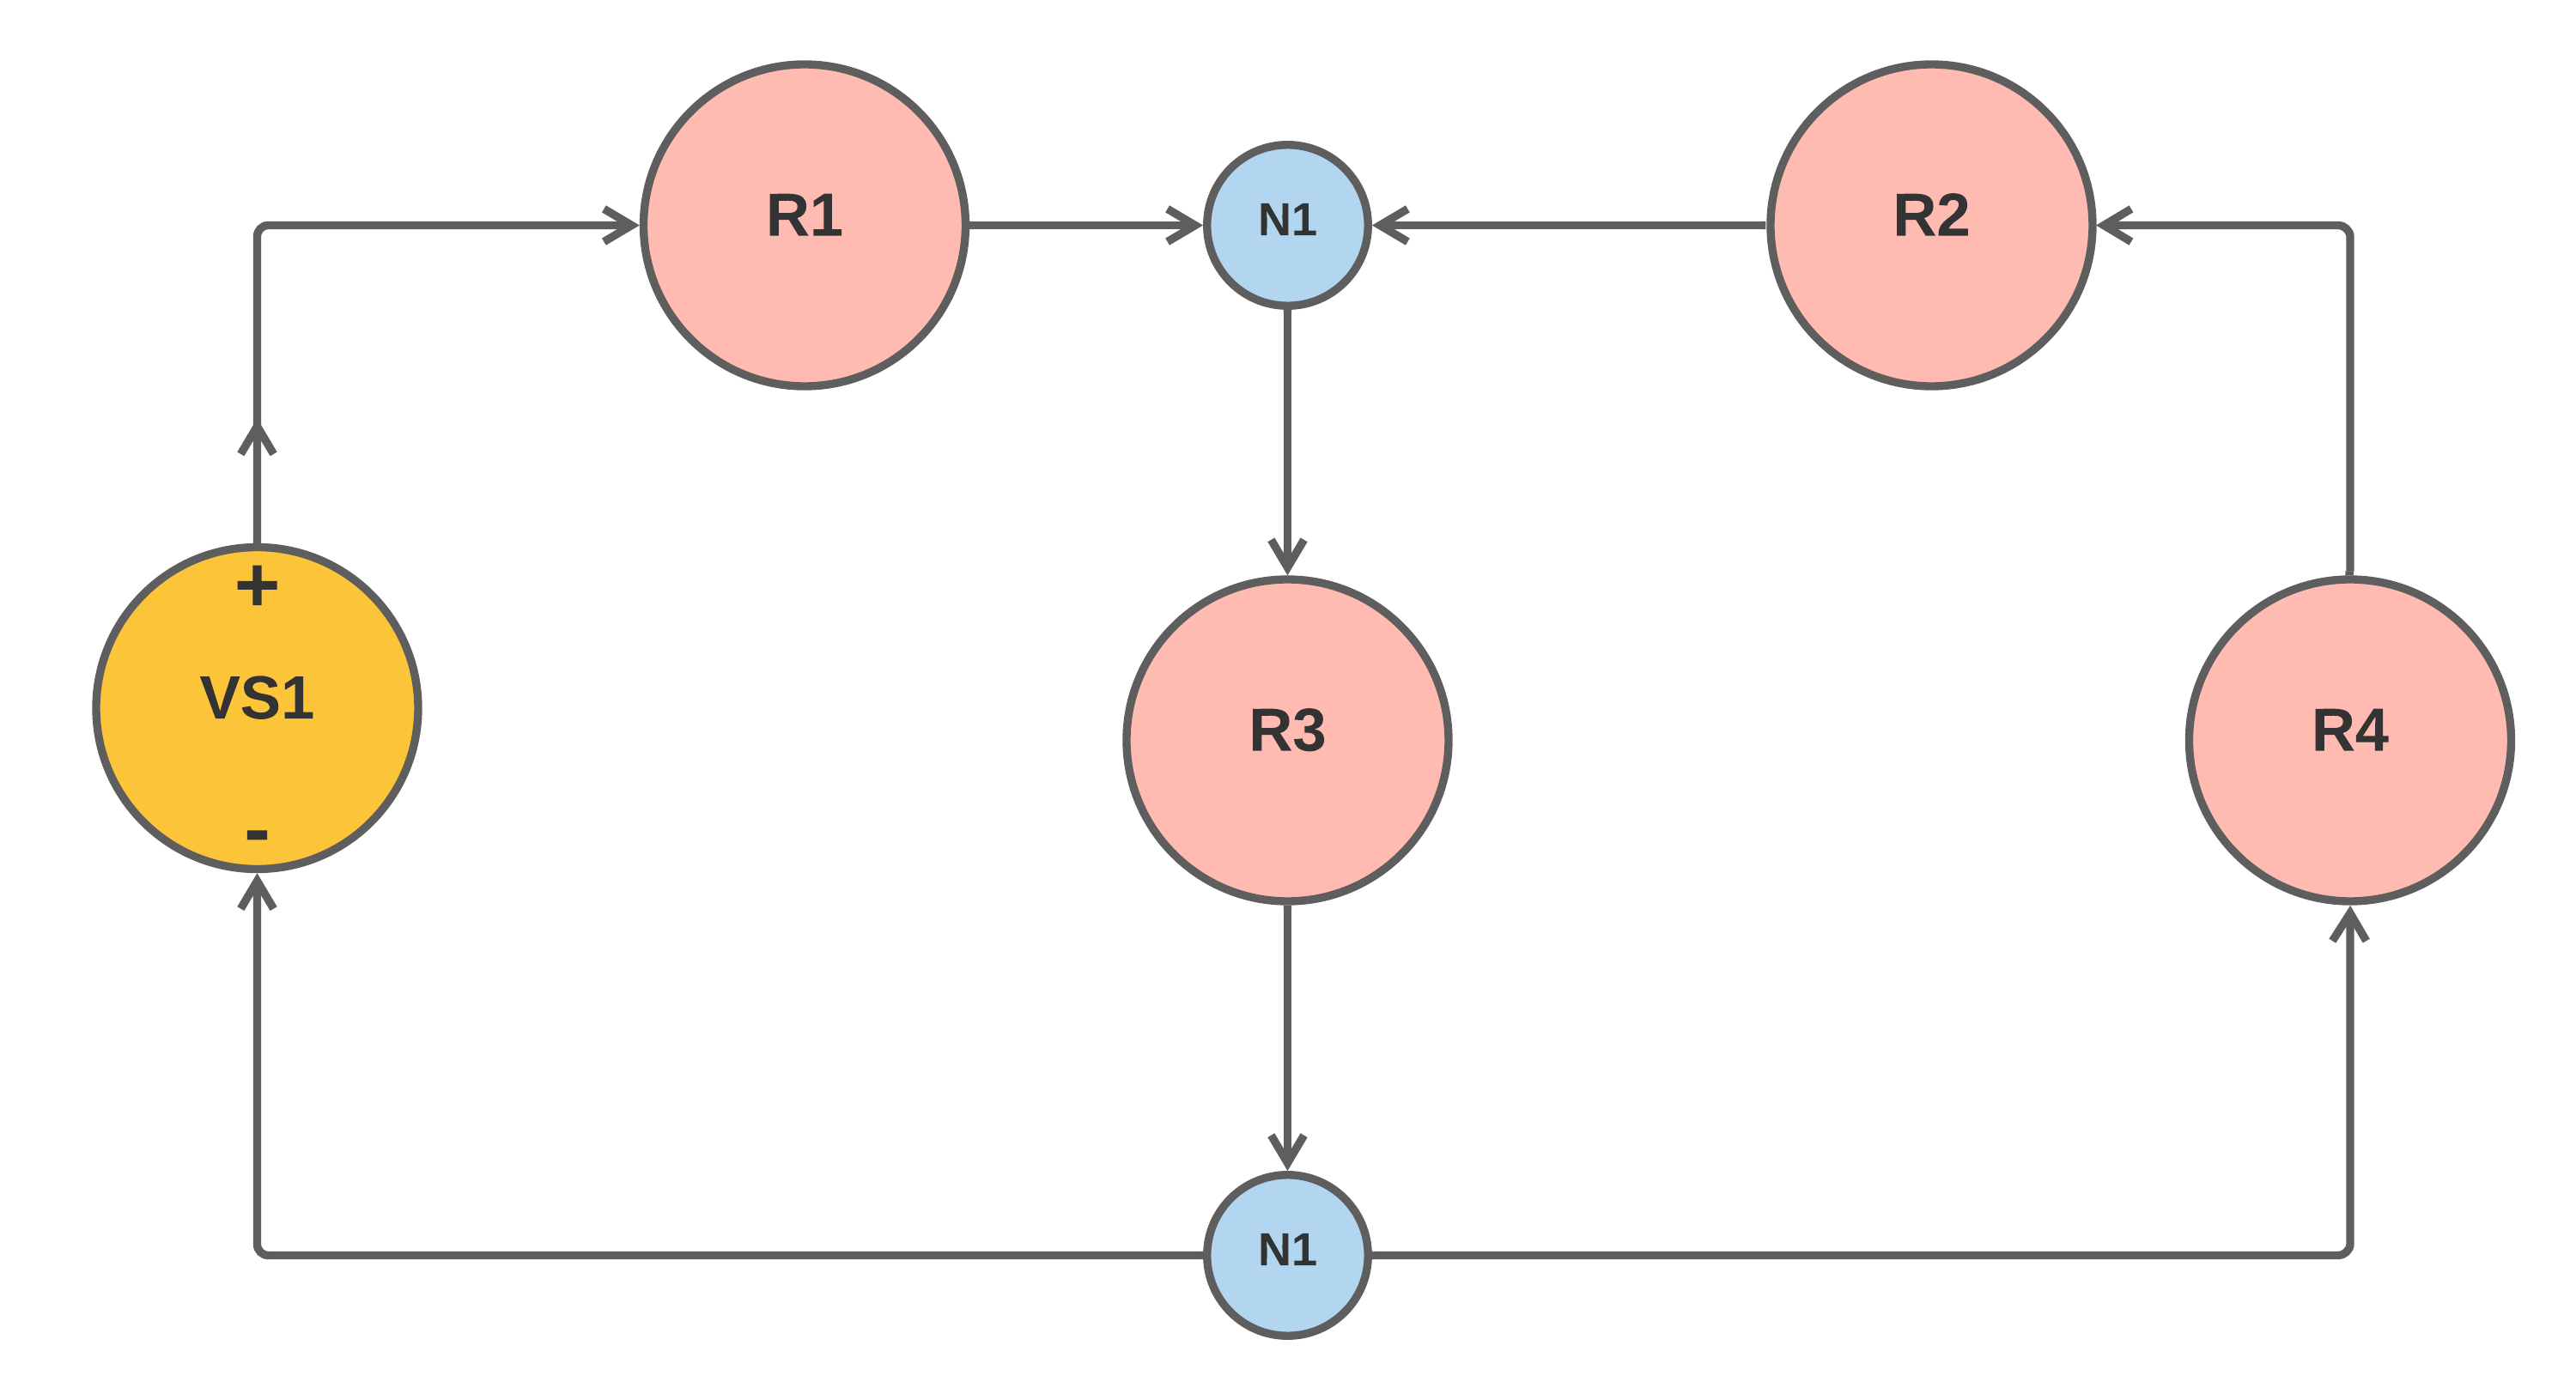
\includegraphics[scale=0.09]{images/Graph_representation.png}
        \caption{Graph representation of the Circuit}
        \label{fig:circuit_graph}
    \end{figure}

    \subsection{Circuit Solving}
    \noindent
    \underline{Input}: Directed Graph representation of the circuit. \\
    \underline{Output}: Current and Voltage Values of each element (only Resistors for now). \\
    Once the circuit has been read and parsed into a Graph, the problem becomes easier to solve. Our implementation is limited to two circuit loops, we find both loops of the circuit. Following that, we generate the matrix for the resistance of the circuit and solve for current: 
    
    \begin{equation}
        \label{eqn:resistance_matrix}
        \mat R = 
        \begin{bmatrix}
        r_{11} && r_{12} \\
        r_{21} && r_{22}
        \end{bmatrix}
    \end{equation}

    Let $r$ be the row of the matrix, the entries on the diagonal correspond to the sum of all resistance values in the $r^{th}$ loop i.e. $r_{11} = R_1 + R_2 + R_3 + \dots + R_n$ where $n$ is the number of resistors in the first loop. For example, in the circuit in figure \ref{fig:circuit_diagram}, $r_{11} = 1000 + 3000 = 4000$ and $r_{22} = 2000 + 2000 = 4000$. The other two values correspond to the resistors that are shared among loops. For this 2D matrix, $r_{ij}$ where $i \neq j$, corresponds to the \textit{negative} sum of all the resistors shared between loops $i$ and $j$.
    
    \noindent
    We can give the matrix treatment to Ohms law and from a linear equation it becomes a matrix equation:
    \begin{equation}
        \label{eqn:Ohm_steroids}
        \mat R \vec I = \vec V
    \end{equation}
    
    \begin{equation}
        \begin{bmatrix}
        r_{11} && r_{12} \\
        r_{21} && r_{22}
        \end{bmatrix}
        \begin{bmatrix}
        I_1 \\ I_2
        \end{bmatrix}
        =
        \begin{bmatrix}
        V_1 \\ V_2
        \end{bmatrix}
    \end{equation}
    \noindent
    For a circuit with only one loop, $I_2$ becomes zero and the values only exist in the first entry of the matrix. Multiplying the matrices in that case will simply give you Ohm's law linear equation. For two loops, the problem is simply one of solving this matrix by calculating them matrix inverse and multiplying that with $\vec V$. There may be instances where there is only one voltage source, in which case $V_2$ is simply zero. For more than one voltage sources in the circuit, they have to be in either one of the loops i.e. connected in series, in which case voltage values are summed.\\
    This method of solving the circuit can easily scales for $n$ loops:
    \begin{equation}
        \begin{bmatrix}
        r_{11} && r_{12} && \dots && r_{1n}\\
        r_{21} && r_{22} && \dots && r_{2n} \\
        \vdots && \vdots && \ddots && \vdots \\
        r_{n1} && r_{n2} && \dots && r_{nn} \\
        \end{bmatrix}
        \begin{bmatrix}
        I_1 \\ I_2 \\  \vdots \\ I_n
        \end{bmatrix}
        =
        \begin{bmatrix}
        V_1 \\ V_2 \\ \vdots \\ V_n
        \end{bmatrix}
    \end{equation}
    
\section{\textbf{Results}}
    The project was divided into two prime components: Representation of circuit details and the analysis of the circuit. The first part has been done before and solved so we did not focus on that aspect too much. Instead we focused our efforts to derive an algorithm, that assuming we have a machine representation of the circuit data, how would we perform the analysis.\\
    \noindent
    The circuit diagram was modelled as a directed graph (\href{https://github.com/estineali/Hand-Drawn-Circuits}{code found here}) and the direction of the edges was based on the flow of voltage in the components. Modelling this as a graph allows us to run graph algorithms on this and makes the problem easier. We break the circuit into meshes using Johnson's Algorithm and form a matrix using both equations. We can then simply use any matrix solving method to solve this matrix. The matrix dimensions are preserved and this allows us the ability to improve and scale this implementation.\\
    \noindent
    
    \begin{figure}[h!]
        \centering
        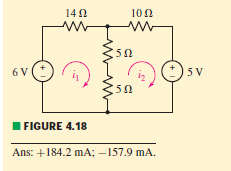
\includegraphics{images/circuit_diag.PNG}
        \caption{The Circuit Diagram}
        \label{fig:circuit_and_answers}
    \end{figure}
    
    \begin{figure}[h!]
        \centering
        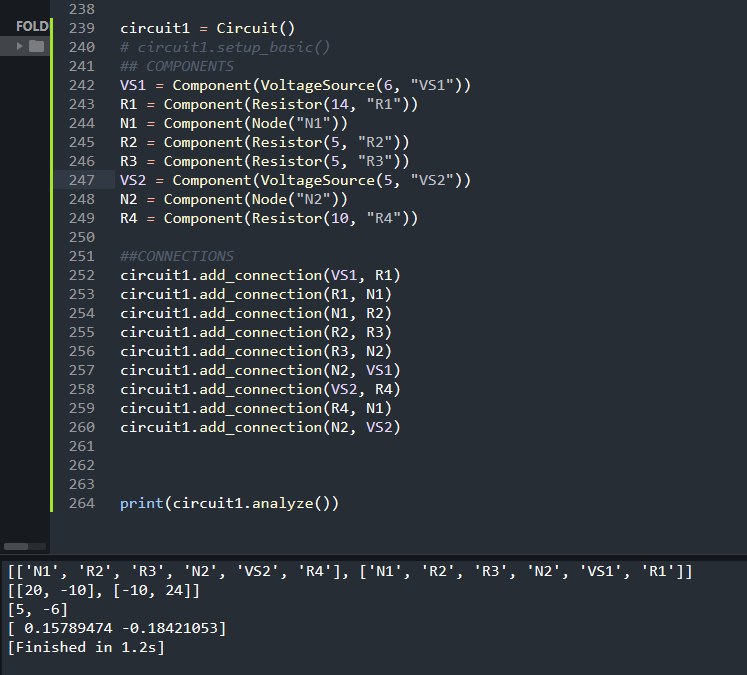
\includegraphics[scale=0.4]{images/results.PNG}
        \caption{Input components into the system.}
        \label{fig:sols_results}
    \end{figure}
    
    The circuit recognition part is trained on a data set of 100 images each of resistors and voltage sources. After taking the image as input, the image goes through the preprocessing stage where it is \textit{converted to gray scale}; training data is also resized to 100x100. The circuit image is then binarized as shown in figure \ref{binarized} and skeletonized (figire \ref{skeletonized} results are not very visible). Following that we perform image segmentation to detect the components and so that we can pass them on to the classifier for further Analysis. 
    
    \begin{figure}[h!]
        \centering
        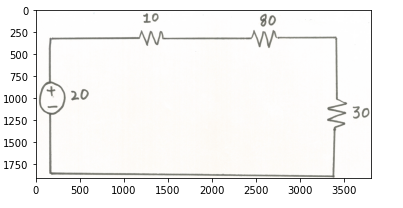
\includegraphics{images/loaded_img.PNG}
        \caption{Loaded Input Circuit Image}
        \label{fig:loaded_img}
    \end{figure}

    \begin{figure}[h!]
        \centering
        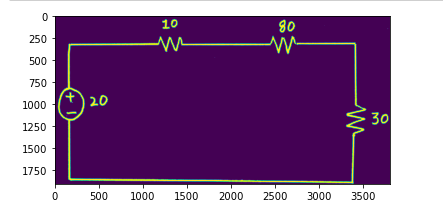
\includegraphics[scale=0.7]{images/handy_binarized.PNG}
        \caption{Binarized input circuit}
        \label{fig:binarized}
    \end{figure}
    
    \begin{figure}[h!]
        \centering
        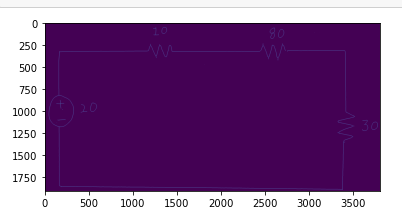
\includegraphics[scale=0.7]{images/skeletonized.PNG}
        \caption{Skeletonized Image}
        \label{fig:Skeletonized}
    \end{figure}
    
    The trained classifier returned 100\% accuracy: 
    
    \begin{figure}[h!]
        \centering
        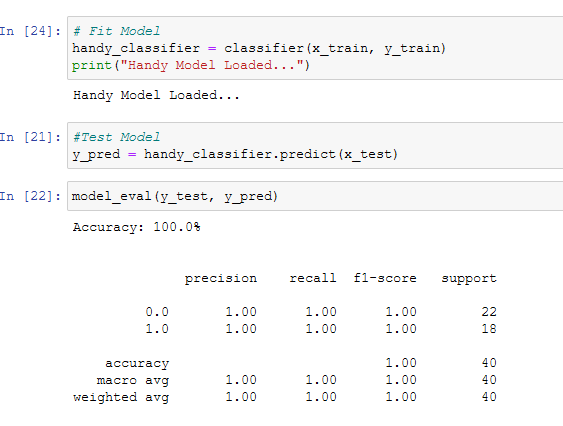
\includegraphics[scale=0.5]{images/metrics.PNG}
        \caption{Classifier metrics: Accuracy, FMeasure}
        \label{fig:Classifier Evaluaton}
    \end{figure}

\newpage

\section{\textbf{Conclusion}}
Further work needs to be done to merge the two components together. We believe with some persistent effort, the analyzer can be scaled to solving meshes of higher mesh complexity. Combining this with the image processing component, we believe the product would be very beneficial. Work on this will be continued. 


\begin{thebibliography}{00}

\bibitem{SIFT}
Larik, M., Ur Rehman, S., and Azeem, S., n.d. \textit{A Tool For Digitizing And Analyzing Hand Drawn Circuit Sketches.}

\bibitem{ANNs}
Mahdi Rabbani, Reza Khoshkangini, H.S. Nagendraswamy, Mauro Conti,
\textit{Hand Drawn Optical Circuit Recognition}, Procedia Computer Science,
Volume 84,
2016,
Pages 41-48,
ISSN 1877-0509,
\href{https://www.sciencedirect.com/science/article/pii/S1877050916300783}{Access Here}

\bibitem{IP_Techs}
S. K. Vasudevan, K. Venkatachalam, S. Anandaram and A. J. Memon, \textit{A Novel Method for Circuit Recognition Through Image Processing Techniques}, Asian Journal of Information Technology, vol. 15, no. 7, pp. 1146-1150, 2016. \href{https://www.scopus.com/inward/record.uri?eid=2-s2.0-84975519853&partnerID=40&md5=079e85950109992c1991a272f31fc35b}{Access Here}

\bibitem{FSM}
L. Naika R, D. R and P. S, \textit{Handwritten Electric Circuit Diagram Recognition: An Approach Based on Finite State Machine}, International Journal of Machine Learning and Computing, vol. 9, no. 3, pp. 374-380, 2020.
\end{thebibliography}
\end{document}
